\iffalse
This file is protected by Copyright. Please refer to the COPYRIGHT file
distributed with this source distribution.

This file is part of OpenCPI <http://www.opencpi.org>

OpenCPI is free software: you can redistribute it and/or modify it under the
terms of the GNU Lesser General Public License as published by the Free Software
Foundation, either version 3 of the License, or (at your option) any later
version.

OpenCPI is distributed in the hope that it will be useful, but WITHOUT ANY
WARRANTY; without even the implied warranty of MERCHANTABILITY or FITNESS FOR A
PARTICULAR PURPOSE. See the GNU Lesser General Public License for more details.

You should have received a copy of the GNU Lesser General Public License along
with this program. If not, see <http://www.gnu.org/licenses/>.
\fi

\def\importpath{}
\input{\importpath snippets/Complex_Mixer_Header}
%----------------------------------------------------------------------------------------
% Update the docTitle and docVersion per document
%----------------------------------------------------------------------------------------
\def\docTitle{Component Data Sheet}
\def\docVersion{1.5}
%----------------------------------------------------------------------------------------
\date{Version \docVersion} % Force date to be blank and override date with version
\title{\docTitle}
\lhead{\small{\docTitle}}

\def\comp{complex\_mixer}
\edef\ecomp{complex_mixer}
\def\Comp{Complex Mixer}
\graphicspath{ {figures/} }

\begin{document}

\section*{Summary - \Comp}
\begin{tabular}{|c|M{13.5cm}|}
	\hline
	\rowcolor{blue}
	                  &                                                    \\
	\hline
	Name              & \comp                                              \\
	\hline
	Worker Type       & Application                                        \\
	\hline
	Version           & v\docVersion \\
	\hline
	Release Date      & 4/2019 \\
	\hline
	Component Library & ocpi.assets.dsp\_comps                              \\
	\hline
	Workers           & \comp.hdl \comp.rcc                                 \\
	\hline
	Tested Platforms  & xsim, isim, modelsim, alst4, ml605, ZedBoard(PL), Matchstiq-Z1(PL), \\
	\hline
\end{tabular}
\input{\importpath snippets/Complex_Mixer_Functionality}
\section*{Worker Implementation Details}
\input{\importpath snippets/Complex_Mixer_HDL_Implementation}
\input{\importpath snippets/Complex_Mixer_RCC_Implementation}
\input{\importpath snippets/Complex_Mixer_Theory}

\section*{Block Diagrams}
\subsection*{Top level}
	\begin{center}
		\begin{tikzpicture}[% List of styles applied to all, to override specify on a case-by-case
				every node/.style={
					align=center,  		% use this so that the "\\" for line break works
					minimum size=2cm	% creates space above and below text in rectangle
				},
				every edge/.style={draw,thick}
			]
			\node[rectangle,ultra thick,draw=black,fill=blue](R2){\Comp};
			\node[rectangle,draw=white,fill=white](R3)[left= of R2]{``in'' \\ Signed complex samples};
			\node[rectangle,draw=white,fill=white](R4)[right= of R2]{``out'' \\ Signed complex samples};
			\node[rectangle,draw=white,fill=white](R5)[above= of R2]{\verb+enable, phs_inc, phs_init+\\ \verb+mag, messageSize+};
			\path[->]
			(R3)edge []	node [] {} (R2)
			(R2)edge []	node [] {} (R4)
			(R2)edge []	node [] {} (R5)
			(R5)edge []	node [] {} (R2)
			;
		\end{tikzpicture}
	\end{center}
	\captionof{figure}{Complex Mixer Top Level Block Diagram}
	\label{fig:block_diagram}

\newpage
\subsection*{State Machine}
	\begin{flushleft}
		Only one finite-state machine (FSM) is implemented by this worker. The FSM supports Zero-Length Messages.
	\end{flushleft}
	{\centering\captionsetup{type=figure}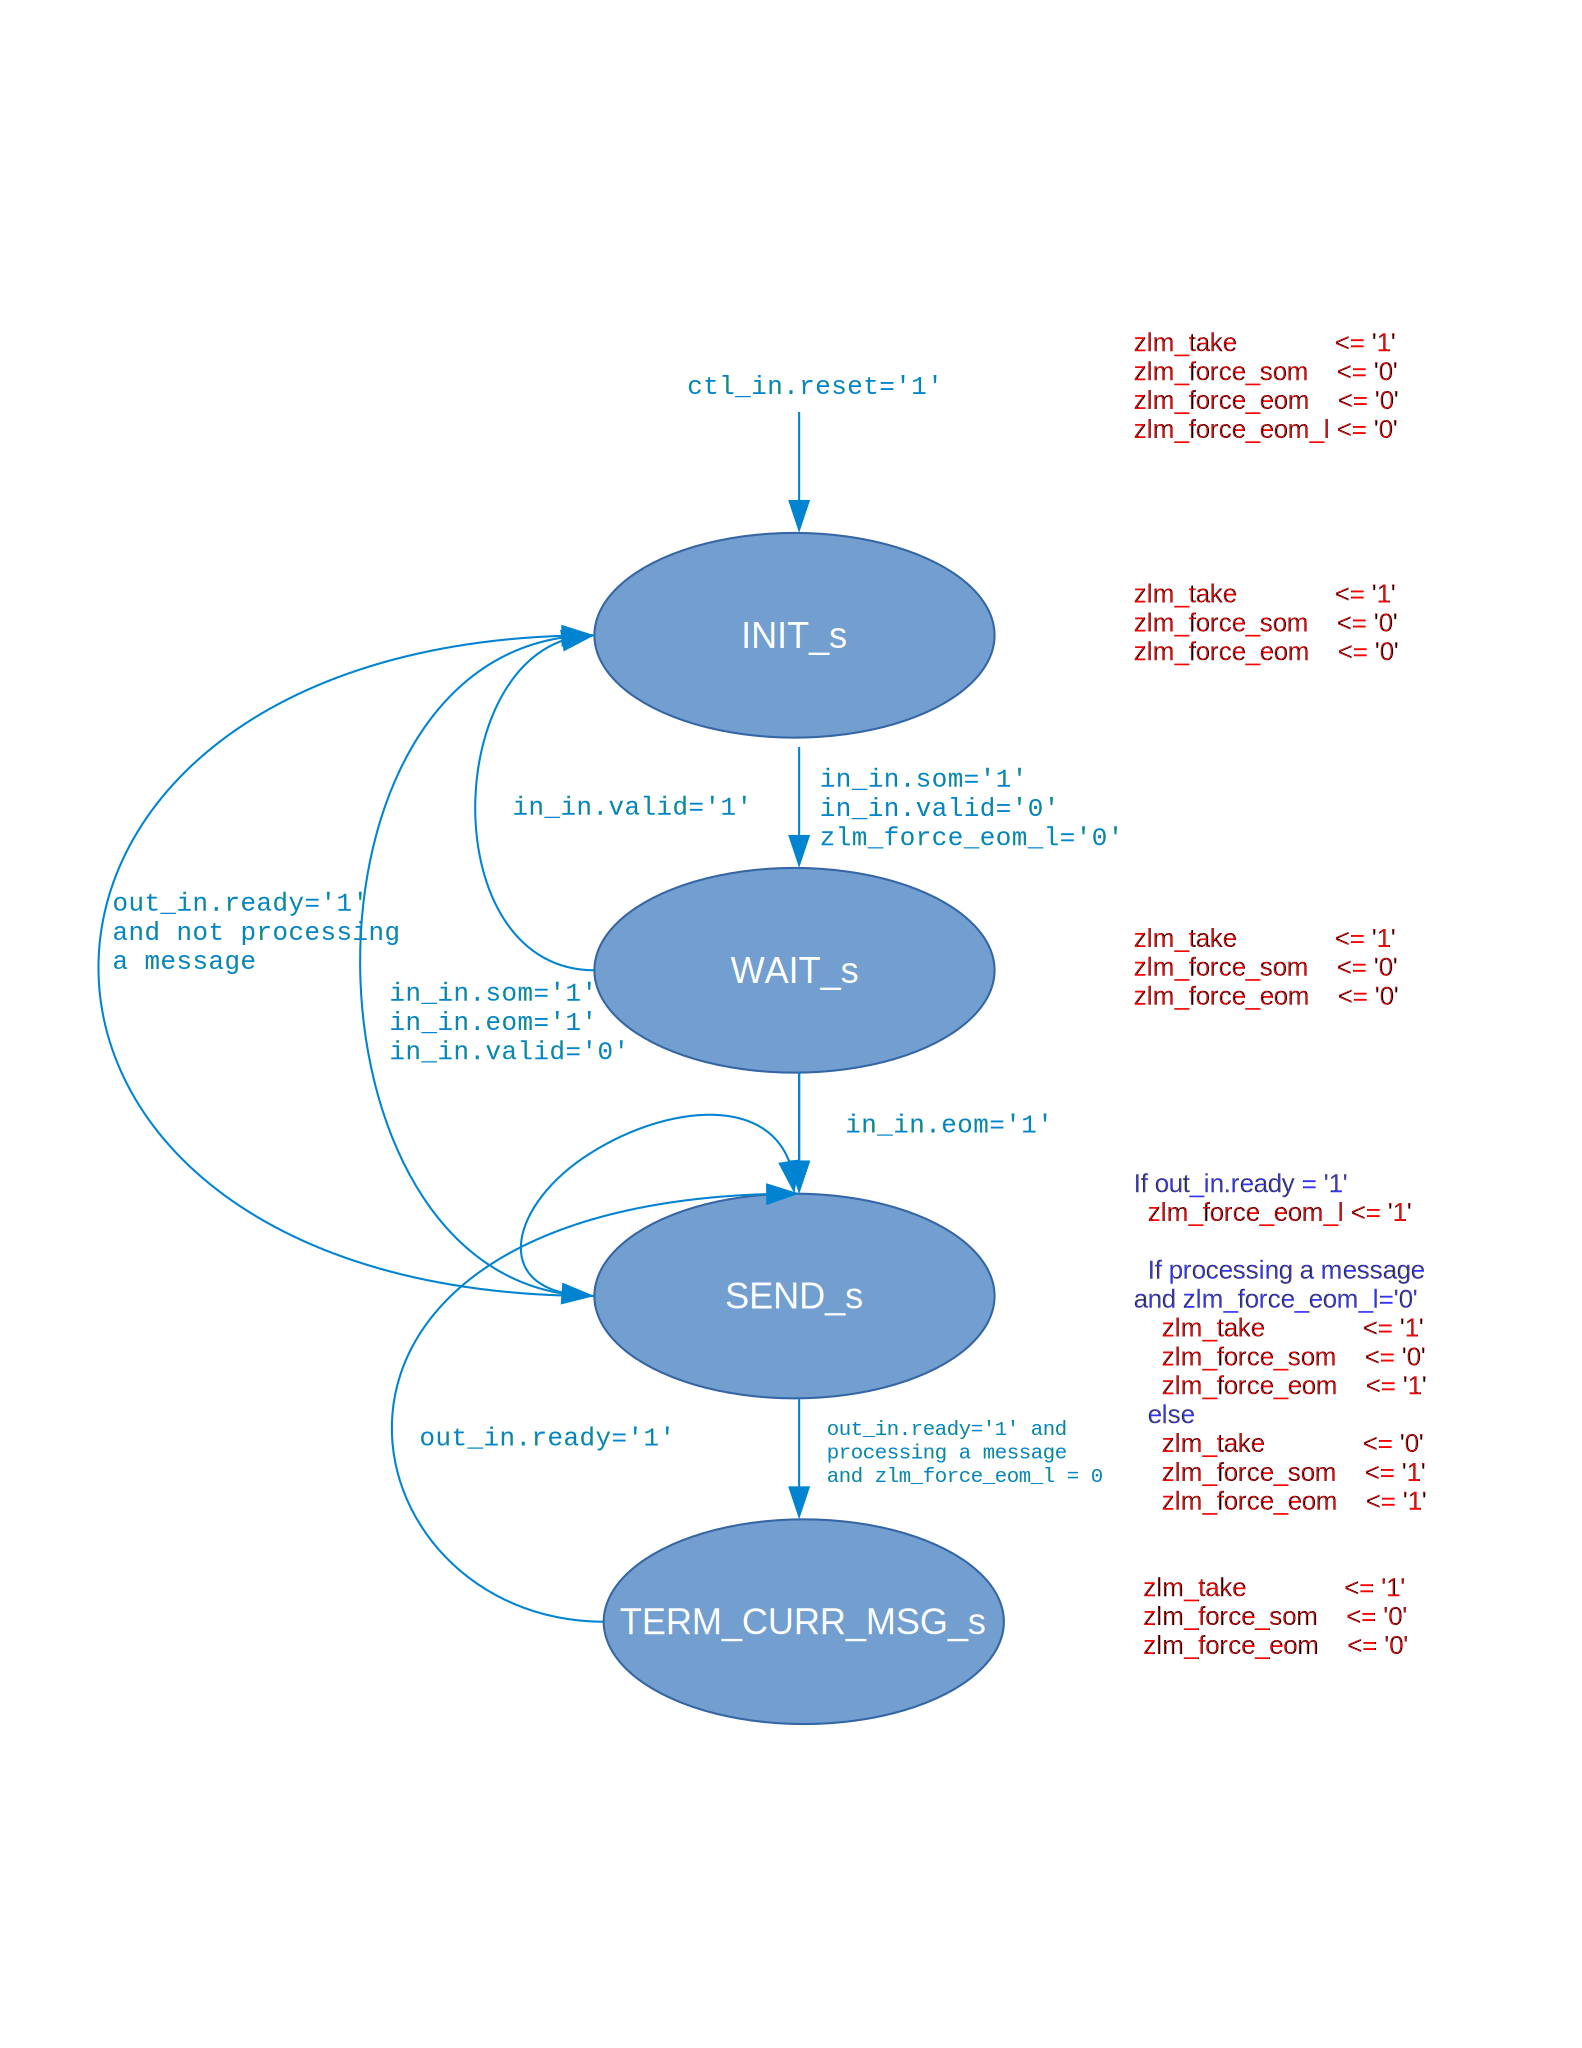
\includegraphics[scale=0.45]{complex_mixer_zlm_fsm}
	\captionof{figure}{Zero-Length Message FSM}
	\label{fig:zlm_fsm}}
        \begin{flushleft}
                Note: In future releases this finite-state machine will be replaced with a register-delay based mechanism, currently exemplified in the dc offset filter
        \end{flushleft}

\newpage
\section*{Source Dependencies}
\subsection*{\comp.rcc}
\begin{itemize}
   \item ocpi-prereq-liquid-1.2.0\_*.rpm and 	ocpi-prereq-liquid-platform-zynq-1.2.0\_*.rpm need to be installed in order to build and run this worker.
   \subitem /opt/opencpi/prerequisites/liquid/include/liquid/liquid.h
\end{itemize}
\subsection*{\comp.hdl}
\begin{itemize}
	\item projects/assets/components/dsp\_comps/complex\_mixer.hdl/complex\_mixer.vhd
        \input{\importpath snippets/Complex_Mixer_Primitive_Dependencies}
\end{itemize}

\begin{landscape}
	\section*{Component Spec Properties}
	\begin{scriptsize}
		\begin{tabular}{|p{3cm}|p{1.5cm}|c|c|c|p{1.5cm}|p{1cm}|p{7cm}|}
			\hline
			\rowcolor{blue}
			Name               & Type   & SequenceLength & ArrayDimensions & Accessibility      & Valid Range & Default & Usage                                                                         \\
			\hline
			\verb+enable+      & Bool   & -              & -               & Readable, Writable & Standard    & true    & Enable(true) or bypass(false) mixer                                           \\
			\hline
			\verb+phs_inc+     & Short  & -              & -               & Readable, Writable & *           & -8192   & Phase increment of NCO \\
			\hline

		\end{tabular}
	\end{scriptsize}

	\section*{Worker Properties}
	\subsection*{\comp.hdl}
	\begin{scriptsize}
		\begin{tabular}{|p{1.5cm}|p{2.5cm}|p{1cm}|c|c|c|p{2cm}|p{1cm}|p{5cm}|}
			\hline
			\rowcolor{blue}
			Type     & Name                      & Type  & SequenceLength & ArrayDimensions & Accessibility       & Valid Range & Default & Usage                                      \\
			\hline
			Property & \verb+CHIPSCOPE_p+        & Bool  & -              & -               & Readable, Parameter & Standard    & false   & Include Chipscope circuit                  \\
			\hline
			Property & \verb+NCO_DATA_WIDTH_p+   & UChar & -              & -               & Readable, Parameter & 12/16       & 12      & Output data width of NCO                   \\
			\hline
			Property & \verb+INPUT_DATA_WIDTH_p+ & UChar & -              & -               & Readable, Parameter & 12/16       & 12      & Input port data width                      \\
			\hline
			Property & \verb+CORDIC_STAGES_p+    & UChar & -              & -               & Readable, Parameter & 16          & 16      & Number of CORDIC stages implemented in NCO \\
			\hline
			Property & \verb+PEAK_MONITOR_p+     & Bool  & -              & -               & Readable, Parameter & Standard    & true    & Include peak monitor circuit               \\
			\hline
			Property & \verb+peak+               & Short & -              & -               & Volatile            & Standard    & -       & Output of peak detector                    \\
			\hline
			Property & \verb+phs_init+    & UShort & -              & -               & Readable, Writable & 0           & 0       & Initial phase of NCO                                                          \\
			\hline
			Property & \verb+mag+         & UShort & -              & -               & Readable, Writable & *           & 1024    & Magnitude of NCO output, which must be in the range \scriptsize\begin{verbatim} [-2^(NCO_DATA_WIDTH_p-1)
   2^(NCO_DATA_WIDTH_p-1)-1]\end{verbatim} in order for the worker to operate properly. \\
			\hline
			Property & \verb+messageSize+ & UShort & -              & -               & Readable, Writable & 8192        & 8192    & Number of bytes in output message                                             \\
			\hline
			Property & \verb+data_select+     & Bool  & -              & -               & Readable, Writable & Standard    & false    & In Bypass Mode: selects data to output: 0=input data, 1=output of NCO   \\
			\hline
		\end{tabular}
	\end{scriptsize}

	\section*{Component Ports}
	\begin{scriptsize}
		\begin{tabular}{|M{2cm}|M{1.5cm}|M{4cm}|c|c|M{9cm}|}
			\hline
			\rowcolor{blue}
			Name & Producer & Protocol           & Optional & Advanced & Usage                  \\
			\hline
			in   & false    & iqstream\_protocol & false    & -        & Signed complex samples \\
			\hline
			out  & true     & iqstream\_protocol & false    & -        & Signed complex samples \\
			\hline
		\end{tabular}
	\end{scriptsize}

	\section*{Worker Interfaces}
	\subsection*{\comp.hdl}
	\begin{scriptsize}
		\begin{tabular}{|M{2cm}|M{1.5cm}|c|c|M{12cm}|}
			\hline
			\rowcolor{blue}
			Type            & Name & DataWidth & Advanced                & Usage                  \\
			\hline
			StreamInterface & in   & 32        & ZeroLengthMessages=true & Signed Complex Samples \\
			\hline
			\rowcolor{blue}
			Type            & Name & DataWidth & Advanced                & Usage                  \\
			\hline
			StreamInterface & out  & 32        & ZeroLengthMessages=true & Signed Complex Samples \\
			\hline
		\end{tabular}
	\end{scriptsize}
\end{landscape}

\section*{Control Timing and Signals}
\begin{flushleft}
	The Complex Mixer HDL worker uses the clock from the Control Plane and standard Control Plane signals.\medskip

	There is a startup delay for this worker. Once the input is ready and valid and the output is ready, there is a delay of \verb+CORDIC_STAGES_p++3 before the first sample is taken. After this initial delay, valid output data is given 2 clock cycles after input data is taken.

	\begin{tabular}{|M{4.5cm}|M{1cm}|M{1cm}|M{1.5cm}|M{2cm}|M{1cm}|M{1cm}|M{2.5cm}|}
		\hline
		\rowcolor{blue}
		Latency         \\
		\hline
		2 clock cycles  \\
		\hline
	\end{tabular}
\end{flushleft}

\begin{landscape}
\section*{Worker Configuration Parameters}
\subsubsection*{\comp.hdl}
%\input{../../\ecomp.hdl/configurations.inc}
\section*{Performance and Resource Utilization}
%\input{../../\ecomp.hdl/utilization.inc}
\end{landscape}
\section*{Test and Verification}
Test cases are derived from the number of properties, and their respective values, as listed in the complex\_mixer-test.xml. Specifically, the \comp.rcc and \comp.hdl implementations tested, as follows:
\begin{itemize}
	\item[1)] Bypass (RCC \& HDL): The input data is forwarded to the output port. For verification of this case, the output file is byte-wise compared to the input file.
	\item[2)] Normal mode (RCC \& HDL): The NCO is configured to tune the input signal to baseband. For verification, an FFT of the output data is performed and the max value of the FFT is checked to be at DC (0 Hz).
%	\item[3)] Bypass mode/data_select=1 : NCO output is captured (HDL)
\end{itemize}
\noindent For all cases, the input file contains a tone of 12.5 Hz sampled at 100 Hz and an amplitude of 32767.\par\medskip

\end{document}
